\documentclass[tikz,border=10pt]{standalone}
\begin{document}
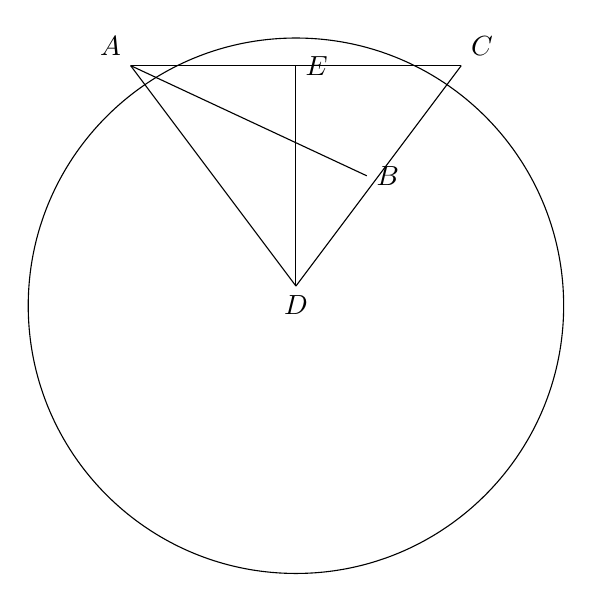
\begin{tikzpicture}[scale=1]

% Coordinates
\coordinate (O) at (0,0);
\coordinate (A) at (-2.1,3.05);
\coordinate (C) at (2.1,3.05);
\coordinate (E) at (0,3.05);
\coordinate (D) at (0,0.25);
\coordinate (B) at (0.9,1.65);

% Circle
\draw (O) circle (3.4);

% Chord and interior segments
\draw (A) -- (C);
\draw (A) -- (D);
\draw (C) -- (D);
\draw (E) -- (D);
\draw (A) -- (B);

% Labels
\node[above left] at (A) {$A$};
\node[above right] at (C) {$C$};
\node[right] at (E) {$E$};
\node[below] at (D) {$D$};
\node[right] at (B) {$B$};

\end{tikzpicture}
\end{document}
